% See: https://latexdraw.com/draw-flowcharts-latex-tutorial/
% See: https://tex.stackexchange.com/questions/51757/how-can-i-use-tikz-to-make-standalone-svg-graphics
\documentclass[crop,tikz,convert={outext=.svg,command=\unexpanded{pdf2svg \infile\space../assets/\outfile}},multi=false]{standalone}

% Required packages
\usepackage{tikz}
\usetikzlibrary{shapes, arrows, calc, positioning}
\pgfmathtruncatemacro\distance{1}

\begin{document}

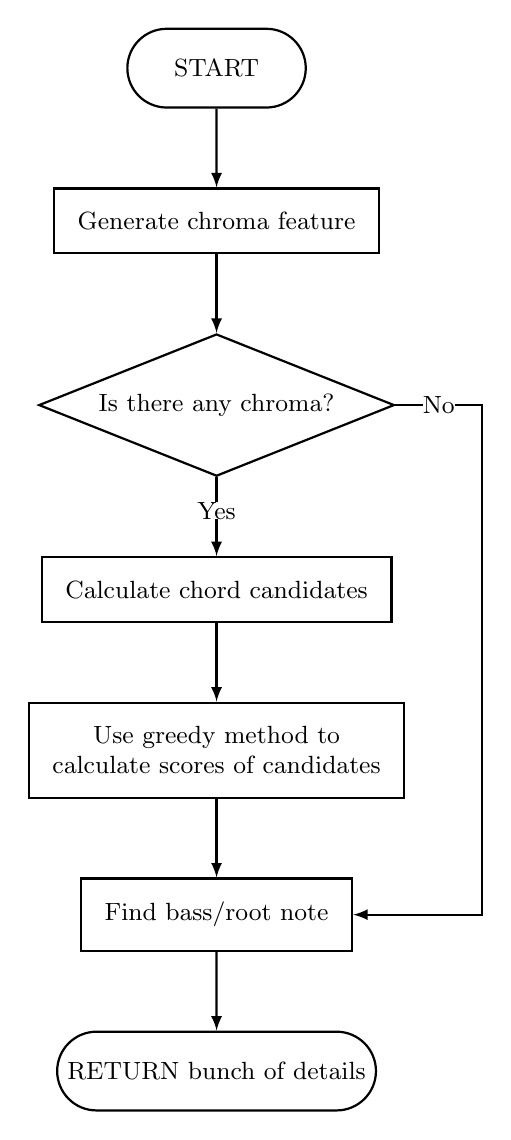
\begin{tikzpicture}[font=\small,thick]

\node[draw,
    rounded rectangle,
    minimum width=2.5cm,
    minimum height=1cm] (block1) {START};

\node[draw,
    align=center,
    below=of block1,
    inner sep=0.3cm] (block2) {Generate chroma feature};

\node[draw,
    diamond,
    below=of block2,
    aspect=2.5,
    align=center,
    minimum width=1cm,
    minimum height=1cm] (block3) {Is there any chroma?};

\node[draw,
    align=center,
    below=of block3,
    inner sep=0.3cm] (block4) {Calculate chord candidates};

\node[draw,
    align=center,
    below=of block4,
    minimum width=2.5cm,
    inner sep=0.3cm] (block5) {Use greedy method to \\ calculate scores of candidates};

\node[draw,
    align=center,
    below=of block5,
    inner sep=0.3cm] (block6) {Find bass/root note};

\node[draw,
    rounded rectangle,
    below=of block6,
    minimum width=2.5cm,
    minimum height=1cm] (block7) {RETURN bunch of details};

\draw[-latex] (block1) -- (block2);
\draw[-latex] (block2) -- (block3);
\draw[-latex] (block3) -- (block4);
\draw[-latex] (block4) -- (block5);
\draw[-latex] (block5) -- (block6);
\draw[-latex] (block6) -- (block7);

\node[below=0.3\distance cm of block3,fill=white,inner sep=0]{Yes};

\draw[-latex] (block3.east) -- +(1.1cm,0)
    node[pos=0.5,fill=white,inner sep=0]{No} |- (block6.east);

\end{tikzpicture}

\end{document}
